\begin{figure}[h]
    \begin{center}
        \begin{adjustbox}{width=0.6\columnwidth}
            \tikzset{every picture/.style={line width=0.75pt}} %set default line width to 0.75pt        
            
            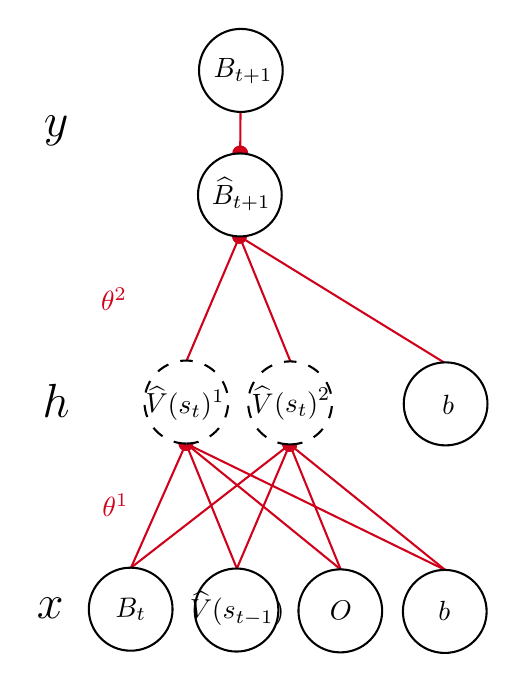
\begin{tikzpicture}[x=0.75pt,y=0.75pt,yscale=-1,xscale=1]
            %uncomment if require: \path (0,350); %set diagram left start at 0, and has height of 350
            
            %Straight Lines [id:da8866607252953388] 
            \draw [color={rgb, 255:red, 208; green, 2; blue, 27 }  ,draw opacity=1 ]   (227.88,279.44) -- (254.36,219.65) ;
            \draw [shift={(254.36,219.65)}, rotate = 293.89] [color={rgb, 255:red, 208; green, 2; blue, 27 }  ,draw opacity=1 ][fill={rgb, 255:red, 208; green, 2; blue, 27 }  ,fill opacity=1 ][line width=0.75]      (0, 0) circle [x radius= 3.02, y radius= 3.02]   ;
            %Straight Lines [id:da0731191645042184] 
            \draw [color={rgb, 255:red, 208; green, 2; blue, 27 }  ,draw opacity=1 ]   (254.68,179.65) -- (280.16,119.85) ;
            \draw [shift={(280.16,119.85)}, rotate = 293.08] [color={rgb, 255:red, 208; green, 2; blue, 27 }  ,draw opacity=1 ][fill={rgb, 255:red, 208; green, 2; blue, 27 }  ,fill opacity=1 ][line width=0.75]      (0, 0) circle [x radius= 3.02, y radius= 3.02]   ;
            %Straight Lines [id:da4826752085294559] 
            \draw [color={rgb, 255:red, 208; green, 2; blue, 27 }  ,draw opacity=1 ]   (304.68,180.05) -- (280.16,119.85) ;
            \draw [shift={(280.16,119.85)}, rotate = 247.84] [color={rgb, 255:red, 208; green, 2; blue, 27 }  ,draw opacity=1 ][fill={rgb, 255:red, 208; green, 2; blue, 27 }  ,fill opacity=1 ][line width=0.75]      (0, 0) circle [x radius= 2.01, y radius= 2.01]   ;
            %Straight Lines [id:da39539248901414714] 
            \draw [color={rgb, 255:red, 208; green, 2; blue, 27 }  ,draw opacity=1 ]   (328.88,280.25) -- (304.36,220.05) ;
            \draw [shift={(304.36,220.05)}, rotate = 247.84] [color={rgb, 255:red, 208; green, 2; blue, 27 }  ,draw opacity=1 ][fill={rgb, 255:red, 208; green, 2; blue, 27 }  ,fill opacity=1 ][line width=0.75]      (0, 0) circle [x radius= 3.02, y radius= 3.02]   ;
            %Straight Lines [id:da8990891706173756] 
            \draw [color={rgb, 255:red, 208; green, 2; blue, 27 }  ,draw opacity=1 ]   (278.88,279.85) -- (254.36,219.65) ;
            \draw [shift={(254.36,219.65)}, rotate = 247.84] [color={rgb, 255:red, 208; green, 2; blue, 27 }  ,draw opacity=1 ][fill={rgb, 255:red, 208; green, 2; blue, 27 }  ,fill opacity=1 ][line width=0.75]      (0, 0) circle [x radius= 3.02, y radius= 3.02]   ;
            %Straight Lines [id:da1147021220204143] 
            \draw [color={rgb, 255:red, 208; green, 2; blue, 27 }  ,draw opacity=1 ]   (328.88,280.25) -- (254.36,219.65) ;
            \draw [shift={(254.36,219.65)}, rotate = 219.12] [color={rgb, 255:red, 208; green, 2; blue, 27 }  ,draw opacity=1 ][fill={rgb, 255:red, 208; green, 2; blue, 27 }  ,fill opacity=1 ][line width=0.75]      (0, 0) circle [x radius= 3.02, y radius= 3.02]   ;
            %Straight Lines [id:da30405558125224674] 
            \draw [color={rgb, 255:red, 208; green, 2; blue, 27 }  ,draw opacity=1 ]   (278.88,279.85) -- (304.36,220.05) ;
            \draw [shift={(304.36,220.05)}, rotate = 293.08] [color={rgb, 255:red, 208; green, 2; blue, 27 }  ,draw opacity=1 ][fill={rgb, 255:red, 208; green, 2; blue, 27 }  ,fill opacity=1 ][line width=0.75]      (0, 0) circle [x radius= 3.02, y radius= 3.02]   ;
            %Straight Lines [id:da7841365763851936] 
            \draw [color={rgb, 255:red, 208; green, 2; blue, 27 }  ,draw opacity=1 ]   (227.88,279.44) -- (304.36,220.05) ;
            \draw [shift={(304.36,220.05)}, rotate = 322.17] [color={rgb, 255:red, 208; green, 2; blue, 27 }  ,draw opacity=1 ][fill={rgb, 255:red, 208; green, 2; blue, 27 }  ,fill opacity=1 ][line width=0.75]      (0, 0) circle [x radius= 3.02, y radius= 3.02]   ;
            %Straight Lines [id:da5618158283475858] 
            \draw [color={rgb, 255:red, 208; green, 2; blue, 27 }  ,draw opacity=1 ]   (379.21,280.52) -- (304.36,220.05) ;
            \draw [shift={(304.36,220.05)}, rotate = 218.93] [color={rgb, 255:red, 208; green, 2; blue, 27 }  ,draw opacity=1 ][fill={rgb, 255:red, 208; green, 2; blue, 27 }  ,fill opacity=1 ][line width=0.75]      (0, 0) circle [x radius= 3.02, y radius= 3.02]   ;
            %Straight Lines [id:da4509011415852858] 
            \draw [color={rgb, 255:red, 208; green, 2; blue, 27 }  ,draw opacity=1 ]   (378.61,180.51) -- (280.16,119.85) ;
            \draw [shift={(280.16,119.85)}, rotate = 211.64] [color={rgb, 255:red, 208; green, 2; blue, 27 }  ,draw opacity=1 ][fill={rgb, 255:red, 208; green, 2; blue, 27 }  ,fill opacity=1 ][line width=0.75]      (0, 0) circle [x radius= 3.02, y radius= 3.02]   ;
            %Straight Lines [id:da7242656967921071] 
            \draw [color={rgb, 255:red, 208; green, 2; blue, 27 }  ,draw opacity=1 ]   (379.21,280.52) -- (254.36,219.65) ;
            \draw [shift={(254.36,219.65)}, rotate = 205.99] [color={rgb, 255:red, 208; green, 2; blue, 27 }  ,draw opacity=1 ][fill={rgb, 255:red, 208; green, 2; blue, 27 }  ,fill opacity=1 ][line width=0.75]      (0, 0) circle [x radius= 3.02, y radius= 3.02]   ;
            %Shape: Ellipse [id:dp9097533963365589] 
            \draw  [fill={rgb, 255:red, 255; green, 255; blue, 255 }  ,fill opacity=1 ][dash pattern={on 4.5pt off 4.5pt}] (304.36,220.05) .. controls (293.22,219.96) and (284.26,210.94) .. (284.35,199.89) .. controls (284.44,188.84) and (293.54,179.96) .. (304.68,180.05) .. controls (315.82,180.14) and (324.77,189.17) .. (324.69,200.21) .. controls (324.6,211.26) and (315.5,220.14) .. (304.36,220.05) -- cycle ;
            %Shape: Ellipse [id:dp9467435778420286] 
            \draw  [fill={rgb, 255:red, 255; green, 255; blue, 255 }  ,fill opacity=1 ][dash pattern={on 4.5pt off 4.5pt}] (254.36,219.65) .. controls (243.22,219.56) and (234.27,210.53) .. (234.36,199.49) .. controls (234.44,188.44) and (243.54,179.56) .. (254.68,179.65) .. controls (265.82,179.74) and (274.78,188.77) .. (274.69,199.81) .. controls (274.6,210.86) and (265.5,219.74) .. (254.36,219.65) -- cycle ;
            %Shape: Ellipse [id:dp4514100854948462] 
            \draw  [fill={rgb, 255:red, 255; green, 255; blue, 255 }  ,fill opacity=1 ] (379.29,220.52) .. controls (368.15,220.43) and (359.2,211.4) .. (359.29,200.36) .. controls (359.37,189.31) and (368.47,180.43) .. (379.61,180.52) .. controls (390.75,180.61) and (399.71,189.64) .. (399.62,200.68) .. controls (399.53,211.73) and (390.43,220.61) .. (379.29,220.52) -- cycle ;
            %Shape: Ellipse [id:dp2836578028815524] 
            \draw  [fill={rgb, 255:red, 255; green, 255; blue, 255 }  ,fill opacity=1 ] (227.56,319.44) .. controls (216.42,319.35) and (207.46,310.32) .. (207.55,299.28) .. controls (207.64,288.23) and (216.74,279.35) .. (227.88,279.44) .. controls (239.02,279.53) and (247.97,288.56) .. (247.89,299.6) .. controls (247.8,310.65) and (238.7,319.53) .. (227.56,319.44) -- cycle ;
            %Shape: Ellipse [id:dp10987171532240936] 
            \draw  [fill={rgb, 255:red, 255; green, 255; blue, 255 }  ,fill opacity=1 ] (278.56,319.85) .. controls (267.42,319.76) and (258.46,310.73) .. (258.55,299.69) .. controls (258.64,288.64) and (267.74,279.76) .. (278.88,279.85) .. controls (290.02,279.94) and (298.97,288.96) .. (298.88,300.01) .. controls (298.79,311.06) and (289.69,319.94) .. (278.56,319.85) -- cycle ;
            %Shape: Ellipse [id:dp5734471221931936] 
            \draw  [fill={rgb, 255:red, 255; green, 255; blue, 255 }  ,fill opacity=1 ] (328.56,320.25) .. controls (317.42,320.16) and (308.46,311.13) .. (308.55,300.09) .. controls (308.64,289.04) and (317.74,280.16) .. (328.88,280.25) .. controls (340.01,280.34) and (348.97,289.37) .. (348.88,300.41) .. controls (348.79,311.46) and (339.69,320.34) .. (328.56,320.25) -- cycle ;
            %Shape: Ellipse [id:dp8405299754625457] 
            \draw  [fill={rgb, 255:red, 255; green, 255; blue, 255 }  ,fill opacity=1 ] (378.89,320.52) .. controls (367.75,320.43) and (358.79,311.4) .. (358.88,300.36) .. controls (358.97,289.31) and (368.07,280.43) .. (379.21,280.52) .. controls (390.35,280.61) and (399.3,289.64) .. (399.21,300.68) .. controls (399.13,311.73) and (390.03,320.61) .. (378.89,320.52) -- cycle ;
            %Straight Lines [id:da531681756338569] 
            \draw [color={rgb, 255:red, 208; green, 2; blue, 27 }  ,draw opacity=1 ]   (280.48,79.86) -- (280.64,59.86) ;
            \draw [shift={(280.48,79.86)}, rotate = 270.46] [color={rgb, 255:red, 208; green, 2; blue, 27 }  ,draw opacity=1 ][fill={rgb, 255:red, 208; green, 2; blue, 27 }  ,fill opacity=1 ][line width=0.75]      (0, 0) circle [x radius= 3.35, y radius= 3.35]   ;
            %Shape: Ellipse [id:dp7122318662628844] 
            \draw  [fill={rgb, 255:red, 255; green, 255; blue, 255 }  ,fill opacity=1 ] (280.64,59.86) .. controls (269.51,59.77) and (260.55,50.74) .. (260.64,39.69) .. controls (260.73,28.65) and (269.83,19.77) .. (280.97,19.86) .. controls (292.1,19.95) and (301.06,28.97) .. (300.97,40.02) .. controls (300.88,51.06) and (291.78,59.95) .. (280.64,59.86) -- cycle ;
            %Shape: Ellipse [id:dp8923679098088735] 
            \draw  [fill={rgb, 255:red, 255; green, 255; blue, 255 }  ,fill opacity=1 ] (280.16,119.85) .. controls (269.03,119.76) and (260.07,110.74) .. (260.16,99.69) .. controls (260.25,88.65) and (269.35,79.77) .. (280.48,79.86) .. controls (291.62,79.94) and (300.58,88.97) .. (300.49,100.02) .. controls (300.4,111.06) and (291.3,119.94) .. (280.16,119.85) -- cycle ;
            
            % Text Node
            \draw (279.05,299.33) node  [rotate=-0.94] [align=left] {$\displaystyle \widehat{V}(s_{t-1})$};
            % Text Node
            \draw (329.04,300.22) node  [rotate=-1.88] [align=left] {$\displaystyle O$};
            % Text Node
            \draw (378.8,300.47) node  [rotate=-359.63] [align=left] {$\displaystyle b$};
            % Text Node
            \draw (380.6,200.87) node  [rotate=-358.65] [align=left] {$\displaystyle b$};
            % Text Node
            \draw (253.92,200.36) node  [rotate=-0.88] [align=left] {$\displaystyle \widehat{V}(s_{t})^1$};
            % Text Node
            \draw (305.05,199.96) node  [rotate=-358.47] [align=left] {$\displaystyle \widehat{V}(s_{t})^2$};
            % Text Node
            \draw (280.95,99.59) node  [rotate=-359.67] [align=left] {$\displaystyle \widehat{B}_{t+1}$};
            % Text Node
            \draw (189,299.2) node  [font=\LARGE,rotate=-0.33]  {$x$};
            % Text Node
            \draw (191.8,199.22) node  [font=\LARGE,rotate=-359.71]  {$h$};
            % Text Node
            \draw (191.84,69.22) node  [font=\LARGE,rotate=-0.13]  {$y$};
            % Text Node
            \draw (220.4,249.43) node  [font=\normalsize,color={rgb, 255:red, 0; green, 0; blue, 0 }  ,opacity=1 ,rotate=-359.94]  {$\textcolor[rgb]{0.82,0.01,0.11}{\theta }\textcolor[rgb]{0.82,0.01,0.11}{^{1}}$};
            % Text Node
            \draw (219.7,149.93) node  [font=\normalsize,color={rgb, 255:red, 208; green, 2; blue, 27 }  ,opacity=1 ,rotate=-359.3]  {$\textcolor[rgb]{0.82,0.01,0.11}{\theta }\textcolor[rgb]{0.82,0.01,0.11}{^{2}}$};
            % Text Node
            \draw (227.72,299.44) node  [rotate=-358] [align=left] {$\displaystyle B_{t}$};
            % Text Node
            \draw (281.85,40.31) node  [rotate=-359.39] [align=left] {$\displaystyle B_{t+1}$};
            
            
            \end{tikzpicture}
        \end{adjustbox}
    \end{center}
\caption{\textbf{Feedforward ANN with a 2-units hidden layer.} The figure represents how a feedforward ANN could be used for estimating $V(s_t)$ given a sequence of observed behaviors ($B$) produced while interacting with an object ($O$). Here $x$ and $h$ are vectors indicating the model's input and the inferred representation.  $y$ indicates both the target and the estimate produced by the model while $b$ is a bias term. The collection of all the red lines indicates the $\Theta$ that the ANN has to estimate while each line represents a single parameter $w$. The circles are computational units (i.e. artificial neurons) whose outputs are given by $Act(\sum_{i=1}^N w_i + b )$. Here, $Act$ is a non-linear function conventionally called activation while $N$ is the dimensionality of the previous layer.}
\label{fig: ffnn}
\end{figure}